\chapter[Classificação de textos jurídicos]{Classificação de textos jurídicos}

Neste capítulo, serão apresentadas as análises dos resultados encontrados.

\section{Qualidade da \textit{pipeline}}

A \textit{pipeline} de extração de dados possui uma complexidade muito alta. O fato de ser necessário dividir os documentos que vieram no formato de volumes, fez com que a confiabilidade nos rótulos das peças fosse baixo.

Por conta disso, foi necessário trabalho humano para reclassificar adequadamente os documentos. Além disso, o processo de extração de dados possibilitou que um mesmo documento, passasse pela pipeline mais de uma vez, ocasionando duplicação do seu registro no banco  de dados.

Mesmo sendo confiável o rótulo gerado pelos especilistas, mudanças nos padrões estabelecidos por eles, fez com que documentos com o mesmo conteúdo recebessem classificações distintas, por exemplo um documento \textit{2017080910001} poderia receber o rótulo Outros e também Despacho de Admissibilidade.

Apesar dos problemas registrados com a \textit{pipeline}, a matriz de correlação utilizando \textit{Spearman}, mostrou que as categorias de documentos não possuem correlação entre si. Com a aplicação da limpeza dos dados, observou-se na Figura \ref{fig:correlacaoPecas}, que a correlação entre as categorias aumentou, mas que ainda assim não é significativa. Esta não correlação é um sinal positivo, indicando que os conjunto de documentos possuem características distintas e que indicam ser separáveis.

\section{Análise dos modelos}

Da Tabela \ref{tab:svmParametros}, percebe-se que os parâmetros sugeridos por \citeonline{wang_baselines_2012} apresentaram os melhores resultados nos diferentes processamentos do texto. Ressalva-se, entretanto que, para o contexto em questão, a técnica BoW sobressaíu-se a de Unigramas. Além de que, a função de núcleo linear de \cite{smola_tutorial_2004} obteve performance superior às demais quando fez-se uso do BoW.

Contrapondo ainda \citeonline{wang_baselines_2012}, a performance do modelo linear foi melhor do que o núcleo polinomial de grau 2. O fato do unigrama ter resultado inferior não impede de a combinação do SVM bi-grama \cite{wang_baselines_2012} se sobressair, entretanto, pode ser um indício que para este conjunto de dados o BoW seja o melhor processamento para o SVM.

Na Figura \ref{fig:acc}, fica claro que do \textit{epoch} 20 em diante, a maior parte dos modelos neurais encontram o problema do \textit{overfitting} e mesmo com o uso em diferentes modelos da rede da técnica de \textit{dropout} \cite{srivastava_dropout:_2014}, não foi o suficiente para mitigar o problema. Com relação a isto, os modelos que se sobressaíram foi o CNN-rand \cite{kim_convolutional_2014}, o MLP, o LSTM \cite{hochreiter_long_1997} e o BLSTM \cite{braz_document_2018}, em que estes modelos não ultrapassaram o valor de acurácia de 98$\%$ no conjunto de treinamento, mantendo bons resultados no de validação.

Notoriamente o modelo VDNN \cite{conneau_very_2017} não obteve boa performance, sendo o mais instável e que gerou os piores resultados. Quanto maior a profundidade da rede de VDNN, mais dados são necessários para seu treinamento \cite{conneau_very_2017}, e como neste trabalho têm-se disponível apenas 4 mil amostras, a consequência foi instabilidade. Nos experimentos em que a arquitetura fora proposta, a quantidade de dados era superior, sendo o menor número de amostras para treino 120.000 no conjunto de dados \textit{AG's new}. Dessa forma, este modelo profundo mostrou-se pouco efetivo na separação de documentos jurídicos com o número de amostras atuais, ainda que tenha chegado em 82$\%$ na acurácia e 81 $\%$ em precisão, revocação no conjunto de teste. 

O modelo que mostrou melhor performance entre os neurais foi o LSTM com os textos pré-processados, chegando a 94$\%$ de acurácia, 93$\%$ de precisão e 95$\%$ de revocação. Além de que seu tempo para predizer as amostras de teste foram na faixa de 1,58 segundos. A combinação de contextos das palavras predecessoras \cite{schuster_bidirectional_1997} não trouxeram tanto ganho de informação com os dados pré-processados. O grande diferencial da BLSTM e BLSTM \cite{braz_document_2018}, foi o fato de serem mais robustas e não demandar o mesmo pré-processamento, sendo sua performance muito próximo ao da LSTM.

Entre os modelos convolucionais, o destaque foi a CNN-rand que foi robusta ao \textit{overfitting} e apresentou bons resultados. Ainda assim, não se obteve a melhor performance deste modelo por sua inicialização ter sido totalmente randômica \cite{kim_convolutional_2014}. O uso de um \textit{embedding} inicial que se reajustasse durante o treinamento aumentaria sua performance \cite{kim_convolutional_2014}, podendo até superar o LSTM. Entretanto, para a língua portuguesa não foi encontrado um \textit{embedding} confiável treinado, optou-se por utilizar a forma randômica do modelo.

O CNN-rand também mostrou-se superior a implementação da CNN \cite{da_silva_document_2018}. A modificação da CNN em adicionar uma camada de MLP com a técnica de \textit{dropout}, reduzindo o tamanho do vocabulário melhorou em 3,2$\%$ na acurácia, 0,67$\%$ na precisão e 3,91$\%$ na revocação comparado a sua implementação original.

Assim como as modificações na CNN melhoraram a performance, o modelo BLSTM foi melhor do que o \citeonline{braz_document_2018}. A adição de uma camada de MLP com \textit{dropout} e o uso da saída de cada neurônio da LSTM na próxima camada, trouxeram o ganho de 10,8$\%$ na acurácia, 14,78$\%$ na precisão e 11,15$\%$ na revocação.

O modelo CNN-LSTM não obteve performance maior do que o LSTM, BLSTM, nem SVM como esperado \cite{zhou_c-lstm_2015}. O BLSTM-C também não foi melhor do que o BoW + SVM e CNN \cite{lai_recurrent_2015}. Assim sendo, neste contexto é melhor escolher e parametrizar uma das duas arquiteturas Recorrente ou Convolucional isoladamente.

\section{Melhores modelos}

Ainda que o estado da arte de classificação de textos tenha avançado bastante na área de modelos neurais, utilizando ainda modelos de atenção \cite{yang_hierarchical_2016,tang_document_2015}, modelos profundos \cite{conneau_very_2017} e demais, o modelo de aprendizado de máquina raso, SVM Linear, performou bem fazendo frente aos modelos do estado da arte, para este conjunto de dados.

\begin{figure}[ht]
    \centering
    \begin{subfigure}[b]{0.45\textwidth}
        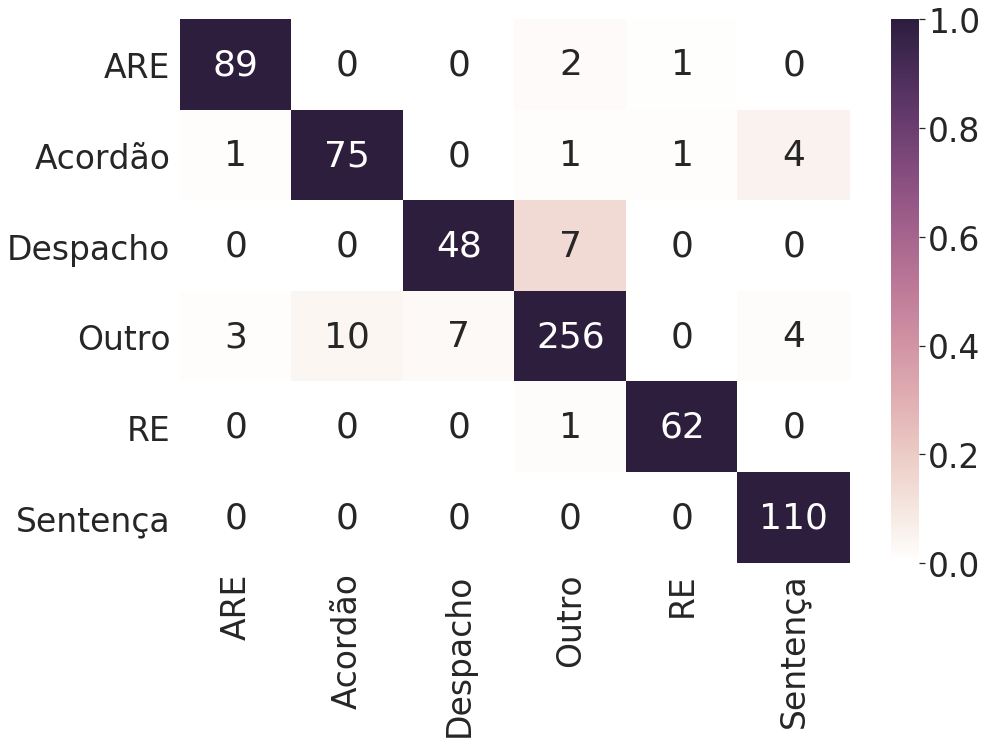
\includegraphics[width=\textwidth]{figuras/matrizCNN}
        \caption{Modelo CNN-rand}
        \label{fig:matrizCNN}
    \end{subfigure}\hfill
    \begin{subfigure}[b]{0.45\textwidth}
        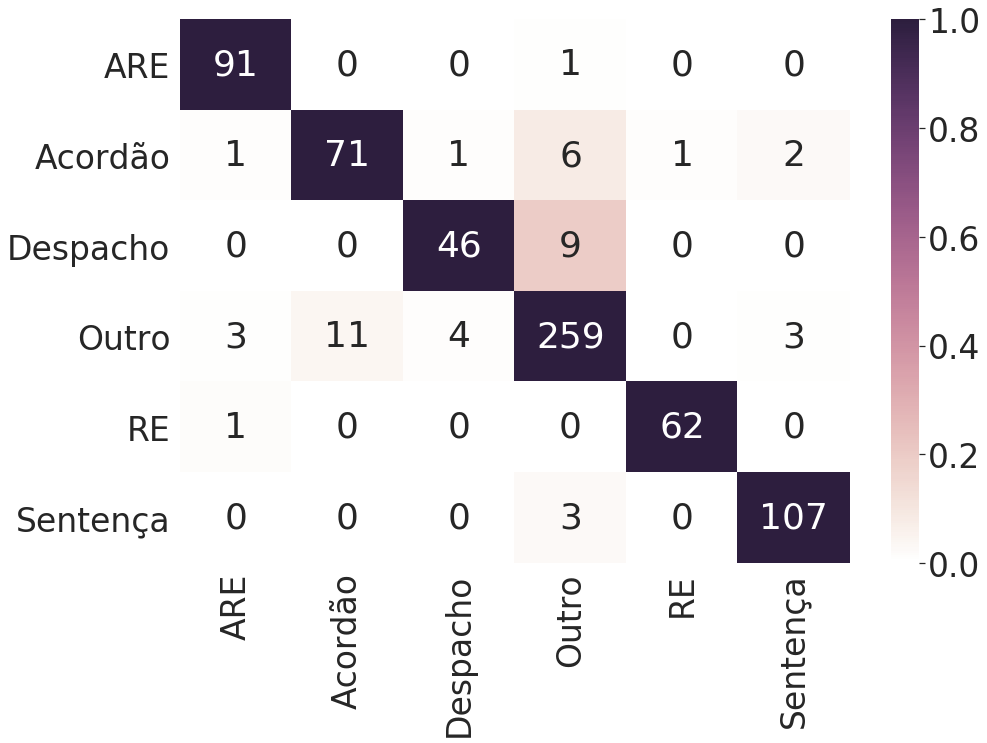
\includegraphics[width=\textwidth]{figuras/matrizBLSTM}
        \caption{Modelo BLSTM}
        \label{fig:matrizBLSTM}
    \end{subfigure}\hfill
    \begin{subfigure}[b]{0.45\textwidth}
        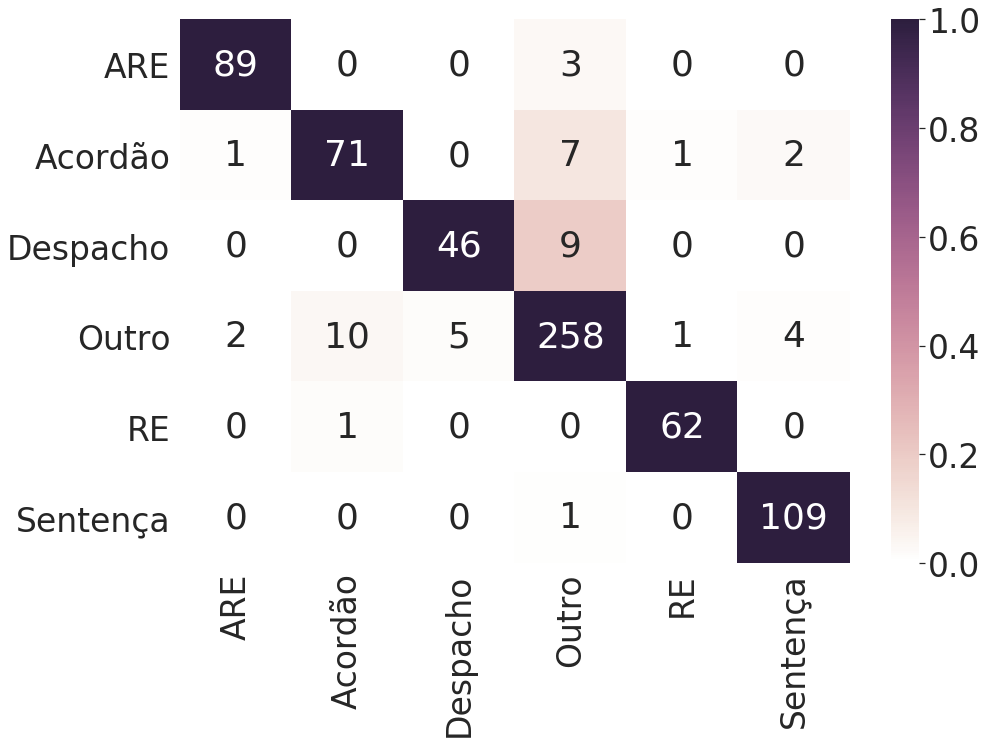
\includegraphics[width=\textwidth]{figuras/matrizSVM}
        \caption{Modelo SVM Linear}
        \label{fig:matrizSVM}
    \end{subfigure}
    
    \caption[Matriz de confusão dos melhores classificadores]{Matriz de confusão dos principais modelos classificadores que obtiveram boas métricas. Fonte: elaboração própria.}
    \label{fig:matrizMelhoresModelos}
\end{figure}

Na Figura \ref{fig:matrizMelhoresModelos}, são apresentadas as matrizes de confusão dos modelos que apresentaram as melhores métricas em relação a: \textbf{tempo de predição}, \textbf{acurácia}, \textbf{precisão} e \textbf{revocação}. A partir destas três matrizes pode-se afirmar que os documentos de peças jurídicas do STF são computacionalmente separáveis, utilizando-se da primeira página de cada um deles. 

Os três modelos confundiram-se de forma semelhante, com as classes Outro e Acordão, Outro e Despacho. Após isto, a confusão foi em classes distintas, como Outro e Sentena na Figura \ref{fig:matrizCNN}; Acordão e Outro na Figura \ref{fig:matrizBLSTM} e \ref{fig:matrizSVM}. De maneira geral, o maior número de confusões foram associadas a categoria Outro. Repara-se que das categorias que apresentaram maior confusão entre si, não são as que apresentaram maiores valores no coeficiente de \textit{spearman} da Tabela \ref{fig:correlacaoPecas}.